\documentclass[a4paper,12pt]{report}

%%%%%%%%%%%%%%%%%%%%%%%%%%%%%%%%%%%%%%%%%%%%%%%%%%%%%%%%%%%%%
%%%%%%                     Packages                    %%%%%%
%%%%%%%%%%%%%%%%%%%%%%%%%%%%%%%%%%%%%%%%%%%%%%%%%%%%%%%%%%%%%


%%%%%%%%%%%%%%%%%%%%%%%%%%%%%%%%%%%%%%%%%%%%%%%%%%%%%%%%%%%%%
%%%%%%                     Packages                    %%%%%%
%%%%%%%%%%%%%%%%%%%%%%%%%%%%%%%%%%%%%%%%%%%%%%%%%%%%%%%%%%%%%

%------------------------------------------------------------
% Impostazioni di base del documento

\usepackage[T1]{fontenc}
\usepackage[utf8]{inputenc} % Codifica utf-8
\usepackage[italian]{babel} % Nomi convenzionali impostati 
%in italiano (chapter,paragraph ec.)
\usepackage{geometry}

%------------------------------------------------------------
% Impostazioni font

%\usepackage[scaled]{helvet}
%\usepackage[familydefault,regular]{Chivo}
%\renewcommand*\familydefault{\sfdefault}

\usepackage{times}

%------------------------------------------------------------
% Impostazioni stile di pagina

\usepackage{geometry}
\usepackage{frontespizio} 
\usepackage{indentfirst}
\usepackage{fancyhdr} % Per formattare lo stile delle pagine
\usepackage{titlesec} % Per formattare l'intestazione dei capitoli
\usepackage{caption}
\usepackage{setspace}

%------------------------------------------------------------
% Impostazioni tabelle

\usepackage{booktabs}
\usepackage{rotating}

%------------------------------------------------------------

%------------------------------------------------------------
% Impostazioni matematica

\usepackage{amsmath}
\usepackage{amssymb}
\usepackage{amsthm}

%------------------------------------------------------------
% Impostazioni colori

\usepackage{color}
\usepackage{colortbl}
\usepackage[dvipsnames]{xcolor}

%------------------------------------------------------------
% Impostazioni collegamenti ipertestuali

\usepackage{url}
\usepackage{hyperref} % Usato per i collegamenti ipertestuali

%------------------------------------------------------------
% Impostazioni dei codici

\usepackage{listings}

%------------------------------------------------------------
% Impostazioni delle figure

\usepackage{rotfloat}
%\usepackage[capposition=top]{floatrow}

%------------------------------------------------------------
% Impostazioni delle boxes

\usepackage[most]{tcolorbox}

%------------------------------------------------------------
% Impostazioni della bibliografia

\usepackage[autostyle,italian=guillemets]{csquotes} \usepackage[backend=biber,style=alphabetic]{biblatex}

%------------------------------------------------------------
% Utilità

\usepackage{lipsum} % Genera testo casuale
\usepackage{ifpdf}
\usepackage{eso-pic}
\usepackage{framed}

%------------------------------------------------------------

%%%%%%%%%%%%%%%%%%%%%%%%%%%%%%%%%%%%%%%%%%%%%%%%%%%%%%%%%%%%%
%%%%%%                      Style                      %%%%%%
%%%%%%%%%%%%%%%%%%%%%%%%%%%%%%%%%%%%%%%%%%%%%%%%%%%%%%%%%%%%%

%%%%%%%%%%%%%%%%%%%%%%%%%%%%%%%%%%%%%%%%%%%%%%%%%%%%%%%%%%%%%
%%%%%%                       Style                     %%%%%%
%%%%%%%%%%%%%%%%%%%%%%%%%%%%%%%%%%%%%%%%%%%%%%%%%%%%%%%%%%%%%

%------------------------------------------------------------
% Margini

\geometry{top=30mm,bottom=30mm}

%------------------------------------------------------------
% Stile titoli dei capitoli

%\titlespacing{\chapter}
%{0pt}
%{0pt}%{-\headsep-11pt}
%{3\baselineskip}
%
%\titleformat{\chapter}[frame]
%{\normalfont}
%{\filright
%\footnotesize
%\enspace \thechapter\enspace}
%{8pt}
%{\Large\bfseries\filcenter}

\titlespacing{name=\chapter} {0pt}{50pt}{20pt}

\titleformat
{name=\chapter}                  % command
[display]                        % shape
{\normalfont\huge\bfseries}      % format
{} % label
{0pt}                           % sep
{\LARGE}[\vspace{1ex}\titlerule]  % before-code    %% adjust 2ex here as you want.

%------------------------------------------------------------
% Stile titoli delle sezioni

%\titleformat{\section}[block]
%{\normalfont%\sffamily
%}
%{\thesection}{\large}{\titlerule\\[.8ex]\bfseries}

\titleformat
{name=\section}                  % command
[block]                        % shape
{\normalfont\large\bfseries}      % format
{} % label
{0pt}                           % sep
{\large}[\vspace{1ex}]  % before-code    %% adjust 2ex here as you want.

%------------------------------------------------------------
% Stile titoli delle sotto-sezioni

\titleformat
{name=\subsection}                  % command
[block]                        % shape
{\normalfont\normalsize\bfseries}      % format
{} % label
{0pt}                           % sep
{\center\normalsize}[\vspace{1ex}]  % before-code    %% adjust 2ex here as you want.

%------------------------------------------------------------
% Stile dei collegamenti

\hypersetup{colorlinks=true,
			filecolor= gray,
			linkcolor= gray,
			urlcolor= gray,
			citecolor=gray,			
			linktocpage}

%------------------------------------------------------------
% Enunciati

\theoremstyle{plain}
\newtheorem{thm}{Theorem}[section]
\newtheorem{cor}[thm]{Corollario}
\newtheorem{lem}[thm]{Lemma}
\newtheorem{prop}[thm]{Proposition}
\theoremstyle{definition}
\newtheorem{defn}{Definition}[chapter]
\theoremstyle{remark}
\newtheorem{oss}{Osservation}

\newenvironment{sistema}%
{\left\lbrace\begin{array}{@{}l@{}}}%
{\end{array}\right.}

%------------------------------------------------------------
% Stile di pagina delle sezioni

\pagestyle{fancy}
\renewcommand{\chaptermark}[1]{\markboth{\emph{\small{Capitolo \thechapter}}}{}}
\renewcommand{\sectionmark}[1]{\markright{\emph{\small{\thesection\ \boldmath#1\unboldmath}}}}
\fancyfoot[C]{\small\thepage}
%\renewcommand{\footrulewidth}{0pt} Ampiezza della linea del piè
\newcommand{\firstpagenumber}{
\clearpage{\pagestyle{empty}\cleardoublepage}
}
\renewcommand{\headrulewidth}{1pt} %Ampiezza della linea della testatina
%\fancyhead[L]{\leavevmode\smash{\protect\includegraphics[scale=0.7]{Immagini/logo}}}
%\fancyhead[R]{\tiny Titolo}

%------------------------------------------------------------
% Ridefinizione dello stile plain

\fancypagestyle{plain}{%
\renewcommand{\headrulewidth}{0pt} %Ampiezza della linea della testatina
\fancyhf{}
\fancyfoot[C]{\small\thepage}}

%------------------------------------------------------------
% Livello di numerazione delle sezioni

\setcounter{secnumdepth}{5}

%------------------------------------------------------------
% Stile delle caption

\captionsetup[table]{labelfont={bf},textfont={small},
justification={raggedright}}
\captionsetup[figure]{labelfont={bf},textfont={small},
justification={raggedright}}

%------------------------------------------------------------
% Stile dei codici (Python)

\definecolor{mygreen}{rgb}{0,0.6,0}
\definecolor{mygray}{rgb}{0.5,0.5,0.5}
\definecolor{mymauve}{rgb}{0.58,0,0.82}

\lstset{ %
  backgroundcolor=\color{white},   % choose the background color; you must add \usepackage{color} or \usepackage{xcolor}; should come as last argument
  basicstyle=\small,        % the size of the fonts that are used for the code
  breakatwhitespace=false,         % sets if automatic breaks should only happen at whitespace
  breaklines=true,                 % sets automatic line breaking
  captionpos=t,                    % sets the caption-position to bottom
  commentstyle=\color{mygreen},    % comment style
  deletekeywords={...},            % if you want to delete keywords from the given language
  escapeinside={\%*}{*)},          % if you want to add LaTeX within your code
  extendedchars=true,              % lets you use non-ASCII characters; for 8-bits encodings only, does not work with UTF-8
  frame=single,	                   % adds a frame around the code
  keepspaces=true,                 % keeps spaces in text, useful for keeping indentation of code (possibly needs columns=flexible)
  keywordstyle=\color{blue},       % keyword style
  language=Octave,                 % the language of the code
  morekeywords={*,...},           % if you want to add more keywords to the set
  numbers=left,                    % where to put the line-numbers; possible values are (none, left, right)
  numbersep=5pt,                   % how far the line-numbers are from the code
  numberstyle=\tiny\color{mygray}, % the style that is used for the line-numbers
  rulecolor=\color{black},         % if not set, the frame-color may be changed on line-breaks within not-black text (e.g. comments (green here))
  showspaces=false,                % show spaces everywhere adding particular underscores; it overrides 'showstringspaces'
  showstringspaces=false,          % underline spaces within strings only
  showtabs=false,                  % show tabs within strings adding particular underscores
  stepnumber=2,                    % the step between two line-numbers. If it's 1, each line will be numbered
  stringstyle=\color{mymauve},     % string literal style
  tabsize=2,	                   % sets default tabsize to 2 spaces
  title=\lstname                   % show the filename of files included with \lstinputlisting; also try caption instead of title
}

% Nomi convenzionali di Codici ed Elenco dei codici
\addto\captionsitalian{%
	\renewcommand{\lstlistingname}{Codice}}
\addto\captionsitalian{%
	\renewcommand{\lstlistlistingname}{Elenco dei codici}}
	
%------------------------------------------------------------
% Stile dei colori

\definecolor{shadecolor}{gray}{0.95}

%------------------------------------------------------------
% Stile delle boxes

\newtcolorbox
{approfondimento}[1]{colback=gray!20,
colframe=gray!80,fonttitle=\bfseries,
title=#1}

\newtcolorbox
{esempio}[1]{colback=yellow!20,
colframe=yellow!50!red!65,fonttitle=\bfseries,
title=#1}

\newtcolorbox
{suggerimento}[1]{colback=blue!20,
colframe=blue!75,fonttitle=\bfseries,
title=#1}

\newtcolorbox
{nota}[1]{colback=green!15,
colframe=green!50!black!80,fonttitle=\bfseries,
title=#1}

%------------------------------------------------------------



%%%%%%%%%%%%%%%%%%%%%%%%%%%%%%%%%%%%%%%%%%%%%%%%%%%%%%%%%%%%%
%%%%%%                    Documento                    %%%%%%
%%%%%%%%%%%%%%%%%%%%%%%%%%%%%%%%%%%%%%%%%%%%%%%%%%%%%%%%%%%%%

\addbibresource{bibliography.bib}

\begin{document}
	
	%\input{frontespizio/frontespizio.tex}
	
	\begin{frontespizio}
		\Universita{di Napoli Federico II}
		\Facolta{Scuola Politecnica e delle Scienze di Base}
		\Corso[Laurea]{Ingegneria Informatica}
		\Logo{Logo}
		\Titoletto{}
		\Titolo{Il controllo di congestione BBR}
		\Candidato{Riccardo Carbone}
		\Annoaccademico{2016-2017}
		\Rientro{1.5cm}
		\NCandidato{Candidati}
		\Punteggiatura{}
	\end{frontespizio}	
	
	\tableofcontents % Generazione dell'indice
	%\listoffigures % Generazione dell'indice delle figure
	%\listoftables % Generazione dell'indice delle tabelle	
	%\lstlistoflistings % Generazione dell'indice dei codici
	
	\chapter{Introduzione}
		Nonostante gli enormi passi avanti che sono stati compiuti nel campo delle tecnologie usate nelle reti di calcolatori, sono ancora molteplici i casi in cui Internet non trasmette le informazioni alle velocità sperate. \bigskip

Eppure molto s’investe nella ricerca e sviluppo, di un’infrastruttura efficiente per la trasmissione dei segnali, che garantisca elevati livelli di delivery rate end-to-end (in ogni normale condizione). \bigskip

Come dunque, si può immaginare, la causa principale non è nè l’uso di tecnologie inadeguate, nè la mancanza di conoscenza nel loro uso. Il reale freno alle potenziali velocità raggiungibili, nasce da una scelta effettuata negli anni '80, quando fu definito il primo schema per il controllo di congestione del protocollo TCP. \bigskip

Tale scelta riguardava l’identificare il fenomeno di congestione (in senso stretto) con il fenomeno di perdita dei pacchetti. \bigskip

Tuttavia, nonostante i due concetti siano molto differenti, al tempo tale scelta aveva senso, solo in virtù delle limitazioni tecnologiche. \bigskip

Oggi anche la migliore versione loss-based di TCP: Cubic (App. A), fa fatica a garantire un delivery rate elevato. Basti pensare che per poter sostenere 10Gbps con un RTT di 100ms, è necessario un tasso di perdita dello 0.000003\%, e con lo stesso RTT ed un tasso di perdita dell’ 1\% sono sostenibili solo 3Mbps \cite[p.~12]{ietf:draft-ietf-tcpm-cubic-05}. \bigskip

Lo scopo di quest'elaborato è dunque quello di presentare un'alternativa per tali approcci, che non sia più basata sull'evento di packet loss, ma esplicitamente sull'evento di congestione. L'alternativa che è stata approfondita è il nuovo controllo di congestione BBR. \bigskip

Prima di iniziare, è lecito far presente che lo sviluppo di tale soluzione è ancora in corso, per cui alcuni aspetti di questa prima versione potrebbero subire delle modifiche nel corso del tempo.		
		
	\chapter{I problemi degli approcci loss-based}
		
In questo primo capitolo, illustreremo come mai un approccio guidato da eventi di packet loss, non riesce a garantire un buon delivery rate. \bigskip

Il primo passo è comprendere le reali potenzialità del delivery rate.

\section{Il limite del delivery rate}

Nel momento in cui due end-point iniziano a comunicare attraverso la rete Internet, i loro pacchetti attraverseranno una serie di collegamenti (link) intermedi, ognuno dei quali sarà caratterizzato da una propria larghezza di banda. \bigskip

%In ogni istante, il path di comunicazione può essere caratterizzato attraverso :

In ogni istante, esiste esattamente un solo bottleneck link: il collegamento con la velocità di trasmissione più bassa. E' dunque necessario adeguarsi alle velocità di quest'ultimo, che pertanto determinerà il limite superiore del delivery rate end-to-end. \bigskip

La seguente figura fornisce un'immagine semplificata ma coincisa, sul ruolo che riveste il bottleneck link nella comunicazione:

\begin{figure}[H]

\center
\caption{Visione semplificata del bottleneck link}

\includegraphics[scale=0.7]{chapters/2_failed/img/bottleneck_link}

\end{figure}

E' fisicamente impossibile per il delivery rate operare al di sopra del bottleneck rate. 

\section{Il sending rate e la congestione di rete}

%\begin{nota}{Nota}
%
%La definizione di congestione presentata in basso, è ricavata da uno scenario semplificato, in cui comunicano un solo mittente ed un solo destinatario. Per i nostri scopi è più che sufficiente. Tuttavia, la semplificazione aiuta il lettore a comprendere in modo rapido le basi e l'essenza della congestione. \bigskip
%
%Non sarà dunque difficile generalizzare anche alla classica situazione che avremo su Internet, dove sono presenti non solo più flussi concorrenti, ma anche bidirezionali. \bigskip
%
%\end{nota}

Dalla definizione del bottleneck rate (\textit{BtlBw}), discende subito la seguente affermazione:

\begin{center}
\label{sending_bottleneck_cons}
\textit{Un sending rate > bottleneck rate porta ad una crescita del bottleneck buffer, con conseguente aumento dei ritardi}
\end{center}

Per poter caratterizzare il ritardo end-to-end introduciamo un altro parametro caratteristico del path di rete, ovvero il Round-trip-propagation-delay (\textit{RTprop}). \bigskip

L'\textit{RTprop} costituisce il minimo ritardo di propagazione, o se si vuole il limite inferiore dell'RTT per una data comunicazione. \bigskip

Ora, il mittente dovrà attendere un RTT prima d'iniziare una seconda fase d'invio. Infatti ricordiamo che l'RTT per un dato pacchetto, è il tempo che intercorre tra la trasmissione e la ricezione del relativo ack. \bigskip

In una fase d'invio:

\begin{itemize}

\item Se il sending rate fosse minore o prossimo al bottleneck rate, il mittente introdurrebbe nella rete un amount inflight\footnote{Quantità di dati inviata dal sender, ma non ancora riscontrata}, tale da non contribuire alla crescita del bottleneck buffer. Per cui in tali condizioni l'RTT = \textit{RTprop}:

\end{itemize}

\begin{figure}[H]

\center
\caption{Delivery rate and round trip time vs inflight part 1}
\label{Delivery_rate_round_trip_time_part_1}
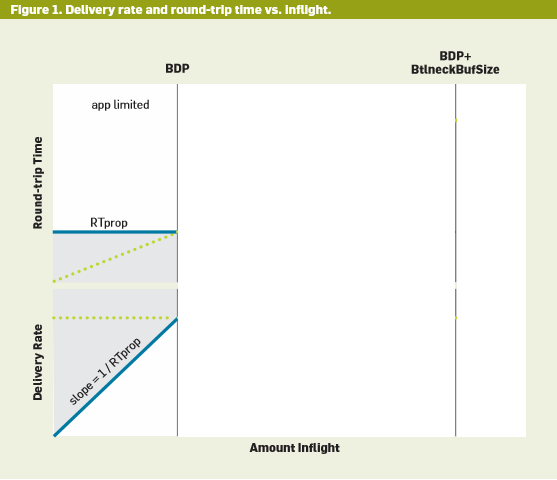
\includegraphics[scale=0.8]{chapters/2_failed/img/Delivery_rate_round_trip_time_part_1}
\caption*{Figura tratta da \cite[p.~60]{Cardwell:2017:BCC:3042068.3009824}}

\end{figure}

\begin{itemize}

\item Se il sending rate fosse superiore al bottleneck rate, il mittente introdurrebbe nella rete un amount inflight superiore alla capacità di quest'ultima. L'RTT aumenta, per via della crescita del bottleneck buffer, e per bilanciare l'amount inflight così da fissare il delivery rate sul bottleneck rate:

\end{itemize}

\begin{figure}[H]

\center
\caption{Delivery rate and round trip time vs inflight}
\label{Delivery_rate_round_trip_time}
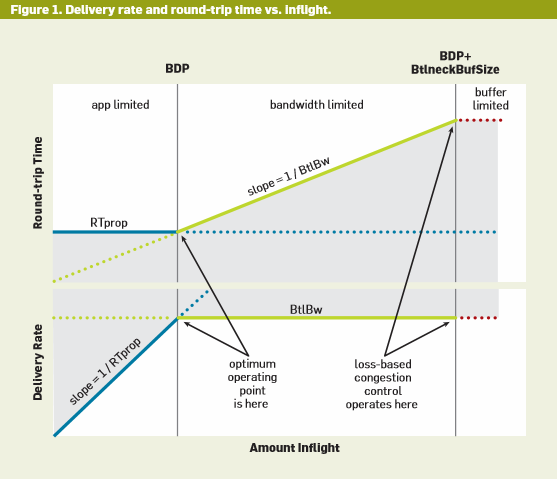
\includegraphics[scale=0.8]{chapters/2_failed/img/Delivery_rate_round_trip_time}
\caption*{Figura tratta da \cite[p.~60]{Cardwell:2017:BCC:3042068.3009824}}

\end{figure}

Questi due casi sono molto importanti, in quanto nel primo il mittente non contribuisce all'aumento dei ritardi, mentre nel secondo si. E' possibile quindi definire la condizione limite, che separa le due situazioni, introducendo il \textit{BDP} (bandwidth delay product \cite[p.~59]{Cardwell:2017:BCC:3042068.3009824}):

\[ BDP \:=\: BtlBw * RTprop \]

Esso definisce la capacità di rete, ovvero il massimo amount inflight che il mittente può introdurre nella rete in un \textit{RTprop}, al massimo delivery rate, senza contribuire nè alla generazione di code, nè all'espansione dei ritardi. \bigskip

\begin{suggerimento}{Osservazione: interpretazione fisica dei parametri caratteristici}

Per fornire una immagine più coincisa di tali parametri, possiamo immaginare una pipe virtuale tra il mittente ed il destinatario. Il \textit{BtlBw} definisce il diametro della pipe, l’\textit{RTprop} la sua lunghezza, mentre il \textit{BDP} la sua capacità (per definizione). \bigskip

\end{suggerimento}

Ora abbiamo tutti gli elementi per comprendere in che condizione il mittente contribuisce ad una congestione di rete, basta trasmettere in un \textit{RTprop} una quantità di dati superiore al \textit{BDP} corrente (pipe overfill). \bigskip

\section{Gli approcci loss based}

Tali approcci limitano il sending rate del mittente, ponendo un limite superiore per l'inflight amount: la congestion window (\texttt{cwnd}). \bigskip

Sulla base delle proprie informazioni locali, l'algoritmo modula la congestion window nel corso del tempo. \bigskip

La modulazione provvede semplicemente ad incrementare la \texttt{cwnd} (ogni versione usa tecniche differenti) , finchè non si verifica o un evento di timeout, o un evento di loss. \bigskip

Nel caso di un timeout, si porta la \texttt{cwnd} al valore minimo, in quanto si assume perso tutto ciò che è stato tramesso (anche il BBR manterrà questo comportamento).
Nel caso di un packet loss, la \texttt{cwnd} subisce un decremento moltiplicativo di un fattore $ \beta $. \bigskip

Quest'approccio non produce un controllo accurato del sending rate. Non è infatti possibile rilevare il momento in cui quest'ultimo eccede il bottleneck rate. \bigskip

Il risultato conseguente sono condizioni operative altalenanti, in cui per la maggior parte si espandono i ritardi, e caricano i buffer intermedi. \bigskip

Per essere più specifici, a seconda delle dimensioni dei buffer intermedi (in particolare del bottleneck buffer), potremmo riscontrare i seguenti problemi:

\begin{itemize}

\item \textit{Shallow buffers} : in virtù della loro piccola dimensione, saranno molto frequenti i fenomeni di perdita. Una strategia AIMD porta a decrementi multipli continui della congestion window, quindi un delivery rate di piccola entità;

\item \textit{Deep buffers} : l'algoritmo reagirà nel momento in cui il bottleneck buffer sarà completamente saturo. L'RTT avrà raggiunto in questa condizione il suo picco massimo: valore che cresce all'aumentare della BtlneckBufSize. 
Quindi nel corso del tempo, è favorita la progressione dei ritardi, e delle perdite.

\end{itemize}

In aggiunta le perdite portano a dedicare parte della banda alle ritrasmissioni. \bigskip

A questo punto è comprensibile la necessità di ricercare una strategia alternativa per limitare il sending rate, che non sia proibitiva in termini di loss rate, e che porti il delivery rate in prossimità del bottleneck rate.
		
	\chapter{Il controllo di congestione BBR}		
		Il comportamento di BBR è dettato da un modello del path di rete, su cui il flusso di pacchetti viaggia. Tale modello traccia l'andamento nel corso del tempo del BtlBw e dell'RTprop. \bigskip

Guidato dal proprio modello il BBR setta i propri parametri di controllo :

\begin{enumerate}

\item \texttt{pacing\_rate}: è il parametro principale dell'algoritmo, e regola il sending rate del mittente nel corso del tempo;

\item \texttt{send\_quantum}: definisce la massima unità di aggregazione per i pacchetti da trasmettere. Utile per diminuire l'overhead della CPU del destinatario.

\item \texttt{cwnd}: non ricopre un ruolo principale, ma continua ad essere il limite superiore per la quantità di dati inflight possibile del sender. 

\end{enumerate}

L'apposita configurazione di tali parametri, permetterà al BBR di operare nel punto operativo migliore (target operating point). Ovvero quello in cui sono soddisfatte le condizioni di :

\begin{itemize}

\item \textit{Rate balance} : il sending rate del mittente ed il bottleneck rate sono perfettamente bilanciati;

\item \textit{Full pipe} : la quantità di dati inflight è uguale al BDP corrente. La pipe opera al 100\%, nulla più, nulla meno;

\end{itemize}

\begin{nota}{Nota: focus sull'installazione del BBR}

Tutto ciò che successivamente diremo dell'algoritmo BBR, riguarda solo il lato mittente TCP. Non è necessario alcun cambiamento nel destinatario TCP per utilizzare quest'algoritmo di controllo di congestione. \bigskip

E' importante però mettere l'accento sul fatto che ciò valga per il TCP che già fa uso di un sistema di ARQ (automatic repeat request). \bigskip

Fondamentalmente il BBR potrebbe essere utilizzato anche da un altro protocollo di livello trasporto, l'importante è che disponga di un sistema di ARQ, in quanto gli ack sono alla base del corretto funzionamento dell'algoritmo.

\end{nota}

\section{Il network path model}

In questa sezione approfondiamo come vengono misurati i parametri caratteristici del network path model.

\subsection{Bottleneck bandwidth} 

Nella regione di bandwidth limited illustrata nel grafico \ref{Delivery_rate_round_trip_time}, il delivery rate è praticamente pari al bottleneck rate, essendo questo il suo limite superiore. Quindi la stima del BtlBw può essere raggiunta attraverso il campionamento del delivery rate. \bigskip

Il tempo con la quale sono generati i campioni utili alla stima è temporizzato dagli ACK ricevuti dal mittente.
Approfondiamo adesso, il processo di generazione dei campioni. (per una trattazione specifica consultare \cite{ietf:draft-cheng-iccrg-delivery-rate-estimation-00}) \bigskip

\subsubsection{L'ack rate}

Un ottimo indice possibile per il delivery rate è l'ack rate, ovvero il tasso di dati riscontrati istantaneamente dal destinatario. \bigskip

Per il suo calcolo è necessario mantenere delle informazioni di stato, per ogni pacchetto, e per la connessione:

\begin{enumerate}

\item \texttt{C.delivered}: quantità di dati riscontrati, fino all’istante \texttt{C.delivered\_time};

\item \texttt{C.delivered\_time}: istante in cui è pervenuto l’ack più recente;

\item \texttt{P.delivered}: valore di \texttt{C.delivered} all’atto della trasmissione di P;

\item \texttt{P.delivered\_time}: valore di \texttt{C.delivered\_time} all’atto della trasmissione di P;

\end{enumerate}

A partire da queste è possibile definire l'espressione dell'ack rate:

\begin{center}

\textit{ack rate \texttt{= (C.delivered - P.delivered) / (C.delivered\_time - P.delivered\_time)}}

\end{center}

E' fondamentale comprendere che l'ack rate è vicino al delivery rate se la quantità di dati riscontrata nel $ \Delta t$ individuato, corrisponde a ciò che effettivamente il mittente trasferisce a destinazione.\bigskip

Fenomeni come la compressione, o soppressione degli ack potrebbero alterare la loro normale temporizzazione, portando a sovrastimare o sottostimare (rispettivamente) il delivery rate \cite{ietf:ack-suppression} \bigskip

La compressione è il principale nemico, in quanto una sovrastima per ragioni chiare avanti, è più pericolosa di una sottostima. \bigskip

\begin{approfondimento}{Approfondimento: significato matematico dell'ack rate}

Mostriamo una possibile sequenza di trasmissione, da parte di un generico sender:

\begin{figure}[H]

\center
\caption{Ack rate determinato in corrispondenza del riscontro per Pkt 3}
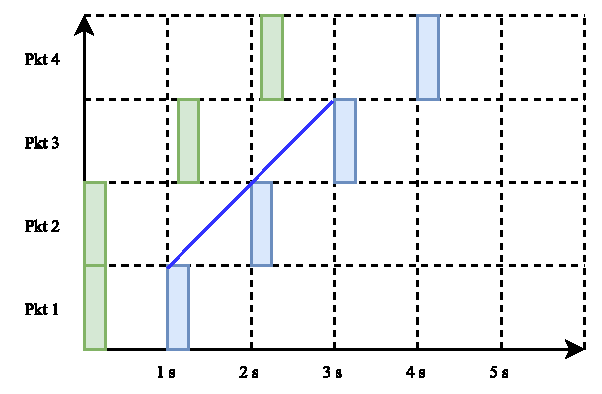
\includegraphics[scale=1.1]{chapters/bbr/img/ack_rate}

\end{figure}

All'atto della ricezione del riscontro per il pacchetto 3, viene determinato l'ack rate come :

\begin{center}

\textit{ack rate = (Pkt3.size + Pkt2.size) / (3s - 1s)}

\end{center}

Dunque l'ack rate rappresenta la pendenza del segmento evidenziato. Ovvero la pendenza con la quale cresce il tasso di dati riscontrati. \bigskip

In aggiunta si fa riflettere che il risultato (considerando pacchetti di dimensione fissa) è 1 pacchetto/secondo. Ed intuitivamente è ciò che ci saremo aspettati come delivery rate. (Ecco perchè l'ack rate è un buon indice in condizioni normali) \bigskip 

\end{approfondimento}

\subsubsection{Il send rate}

Per valutare la veridicità dell'ack rate, viene introdotto il send rate. \bigskip

Ancora una volta per la sua determinazione abbiamo bisogno di mantenere delle informazioni di stato (ulteriori alle precedenti), per ogni pacchetto:

\begin{enumerate}

\item \texttt{P.first\_sent\_time}: istante in cui è iniziata la trasmissione dell’ultimo pacchetto, riscontrato dall’ack ricevuto al tempo \texttt{P.delivered\_time} (a monte dell’invio di P) 
\item \texttt{P.sent\_time}: istante in cui parte la trasmissione del pacchetto

\end{enumerate}

A partire da queste definiamo l'espressione del send rate:

\begin{center}
 
\textit{send rate = \texttt{ (C.delivered - P.delivered) / (P.sent\_time - P.first\_sent\_time)}}

\end{center}

La differenza con l'ack rate sta nell'intervallo di tempo considerato. Il send time rappresenta il tempo che trascorso tra la trasmissione dell'ultimo pacchetto riscontrato, e il pacchetto attualmente riscontrato. \bigskip

Questo permette che il $\Delta t$ considerato includa il tempo di trasmissione dei dati riscontrati. Il send time è in generale >= dell'effettivo tempo di trasmissione. Così è possibile evitare il problema delle sovrastime dell'ack rate. \bigskip

\begin{esempio}{Esempio: un caso di compressione degli ack}

Mostriamo una possibile sequenza di trasmissione, in cui si verifica una compressione degli ack ricevuti:

\begin{figure}[H]

\center
\caption{Fenomeno di compressione degli ack}
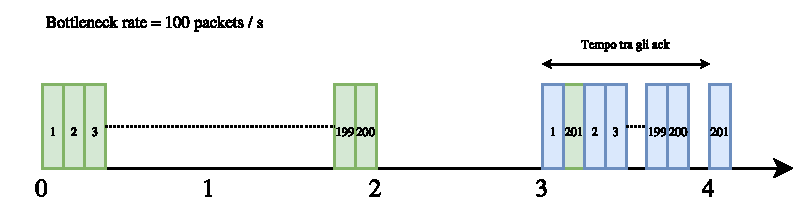
\includegraphics[scale=0.9]{chapters/bbr/img/ack_rate_overstimate.pdf}

\end{figure}

Come si nota dalla figura gli ack per i pacchetti 2-200 vengono ritardati e compressi, ed arrivano in burst tra la trasmissione del pacchetto 201 ed il relativo ack. \bigskip

Ciò porta l'ack rate ad essere 200 packets/s, ma si comprende bene che tra 3s e 4s il sender non ha trasferito 200 pacchetti a destinazione. Quindi in tale situazione l'ack rate non è un indice veritiero del delivery rate. \bigskip

Il reale tempo che i 200 pacchetti impiegano per arrivare al destinatario è di 2s. \bigskip

In questo caso il send rate è di 60 packets/s, perchè considera il tempo trascorso dalla trasmissione del pacchetto 1, a quella del pacchetto 201. Il secondo in più è dovuto all'inclusione del secondo tra 2 e 3 secondi, in cui il mittente è inattivo. \bigskip

Confrontando quindi il send rate e l'ack rate si comprende che il destinatario non può aver ricevuto 200 pacchetti tra 3s e 4s.

\end{esempio}

\begin{approfondimento}{Approfondimento: significato matematico del send rate}

Consideriamo la stessa sequenza di trasmissione precedente, da parte di un generico sender:

\begin{figure}[H]

\center
\caption{Send rate determinato in corrispondenza del riscontro per Pkt 4}
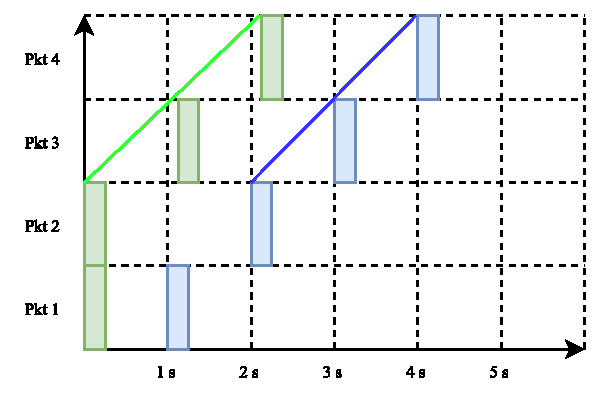
\includegraphics[scale=1.1]{chapters/bbr/img/send_rate}

\end{figure}

All'atto della ricezione del riscontro per il pacchetto 4, viene determinato il send rate come : \bigskip

\begin{center}

\textit{send rate = (Pkt3.size + Pkt4.size) / (2s - 0s)}

\end{center}

Dunque il send rate rappresenta la pendenza del segmento evidenziato in verde. Ovvero la pendenza con la quale cresce il tasso di dati trasmessi. \bigskip 

\end{approfondimento}

\subsubsection{Stima del BtlBw}

Ad ogni ack sarà generato un campione relativo al delivery rate come segue:

\begin{lstlisting}[caption=Delivery rate evaluation]
	time_elapsed = max(send_time,ack_time)
	delivery_rate = data_acked / time_elapsed
\end{lstlisting}

Non ci resta altro che scoprire come da tali campioni venga ottenuta una stima del bottleneck rate. \bigskip

Per poter far questo BBR usa un BtlBwMaxFilter, un windowed filter, di ampiezza $ W_{B} $ :

\[
	\widehat{BtlBw_{T}} \: = \: max(deliveryRate_{t}) \; \forall t\: \in \: [T-W_{B},T]  
\]

L'ampiezza $ W_{B} $ è misurata in multipli di RTprop, e deve essere:

\begin{itemize}

\item Abbastanza estesa da contenere un ProbeBW cycle gain (sezione \ref{ProbeBW}). Così che essa contenga dei sample raccolti nella regione di bandwidth limited, che è effettivamente l'unica regione in cui la stima potrà essere corretta;

\item Abbastanza estesa da combattere l'eventuale presenza di rumore, introdotta da eventuali code lungo il percorsa;

\item Abbastanza corta da poter permettere una pronta a reazione ad una diminuzione del bottleneck rate;

\end{itemize} 

Un ottimo valore è costituito da 10 RTprops. \cite[p.~61]{Cardwell:2017:BCC:3042068.3009824}

\subsection{Round Trip propagation delay}

Per la stima dell'RTprop siamo aiutati dal fatto che il protocollo TCP, già effettua un campionamento dell'RTT, per la gestione dei timeout di ritrasmissione. \bigskip

Anche per determinare RTprop BBR usa un windowed filter, RTpropMinFilter, di ampiezza $ W_{R} $ :

\[
	\widehat{RTprop_{T}} \: = \: min(RTT_{t}) \; \forall t\: \in \: [T-W_{R},T]  
\]

L'ampiezza $ W_{R} $ è misurata in secondi, e deve essere :

\begin{itemize}

\item Estesa almeno quanto un ProbeRTTInterval (sezione \ref{ProbeRTT}). Così che essa contenga dei sample raccolti nella regione di application limited, che è effettivamente l'unica regione in cui la stima potrà essere corretta;

\item Abbastanza estesa da evitare una consistente diminuzione del delivery rate raramente (sezione \ref{ProbeRTT});

\item Abbastanza estesa da poter sfruttare gli istanti in cui l'applicazione limita il delivery rate del mittente, per poter aggiornare la stima dell'RTprop senza diminuire fortemente il delivery rate;

\item Abbastanza corta da poter permettere una pronta reazione ad un variazione dei ritardi;

\end{itemize}

\section{I parametri di controllo}

Compreso in primo luogo come il BBR mantenga aggiornato il modello del network path. Vediamo ora di approfondire i parametri di controllo, usati da quest'ultimo per portarsi nel target operating point.

\subsection{Pacing rate}

Il pacing rate del BBR costituisce un parametro importantissimo (e primario), con cui vengono incontrate nel tempo le condizioni di \textit{Rate balance}, e di \textit{Full pipe}. \bigskip

Effettuare il pacing dei pacchetti significa equi-distanziare le loro trasmissioni. Quindi a monte dell'invio di un dato pacchetto il successivo sarà trasmesso al tempo:

\begin{center}

\textit{nextSendTime = now + packet.size / pacing rate}

\end{center}

Ciò porta ad un adattamento del tasso di trasmissione del mittente al pacing rate, nonostante la capacità del proprio link d'ingresso possa essere superiore. La spaziatura definisce dunque le pause adatte, per sincronizzare il sending rate come voluto. \bigskip

Il set di tale parametro (così come gli altri) avviene ad ogni ack, e può essere riassunto con il seguente pseudocodice:

\begin{lstlisting}[caption=BBRSetPacingRate]
BBRSetPacingRate():
	BBRSetPacingRateWithGain(BBR.pacing_gain)

BBRSetPacingRateWithGain(pacing_gain):
	rate = pacing_gain * BBR.BtlBw
	if (BBR.filled_pipe || rate > BBR.pacing_rate)
		BBR.pacing_rate = rate

\end{lstlisting}

Da cui come ci si aspettava il pacing rate è settato proporzionalmente al BtlBw, attraverso il pacing gain.
La condizione dell'if non ne permette il decremento, in condizioni di pipe underfilled. \bigskip

Un valore di pacing gain pari 1 può permettere di operare nel target operating point, se non sono state formate code in precedenza. Un valore di pacing gain > 1 è utile per ottenere sample utili alla stima del BtlBw, in quanto viene saturato il delivery rate. Ed infine un valore di pacing gain < 1, può essere utilizzato per svuotare le code generate, ed uscire da una situazione di pipe overfill.

\subsection{Send quantum}

Rappresenta la massima unità di aggregazione per i pacchetti inviati dal mittente. Permette quindi d'inviare gruppi di pacchetti in un unico burst, diminuendo l'overhead della CPU del destinatario. \bigskip

Settato ad ogni ack, il suo valore dipende fortemente dal pacing rate. Per valori alti di quest'ultimo, è possibile usare alti valori di send quantum, mentre per valori bassi è meglio diminuire questo ultimo, in quanto creerebbe un aumento dei ritardi, e code lungo il percorso.

\subsection{Congestion window}

La cwnd impone un limite alla quantità di dati inflight del mittente. Nonostante il parametro principale del BBR per il controllo del sending rate sia il pacing rate, la cwnd è molto utilizzata nelle situazioni in cui si vuole subito portare il limite inflight in un particolare punto. Verrebbe speso un maggior tempo se si usufruisse del pacing rate. \bigskip

Per la sua gestione vengono definiti un upper ed un lower bound:

\begin{itemize}

\item \textit{target cwnd}: limite superiore della cwnd, ottenuto in funzione del $ \widehat{BDP} $ (BDP stimato) come:

\textit{target cwnd = cwnd gain * $ \widehat{BDP} $}

\item \textit{BBRMinPipeCwnd}: limite inferiore della cwnd, tipicamente tale da consetire l'invio di 2/4 pacchetti al mittente.

\end{itemize}

Tali limiti sono da considerare strettamente rigidi in condizioni normali (non occorrono nè eventi di loss, nè di timeout). \bigskip

Discutiamo adesso della modulazione del parametro in tali condizioni. \bigskip

Se la pipe è piena, è molto probabile si sia raggiunto il target. Dunque si provvede ad incrementare la cwnd solo se essa non supererà il target. In caso contrario resterà fissata su quest'ultimo. \bigskip 

Invece se siamo al di sotto del target, avviene un semplice incremento pari alla quantità di dati consegnati a destinazione. \bigskip

In ogni caso viene sempre garantito il rispetto del lower bound. \bigskip

Tuttavia, come è ben noto, gli eventi di packet loss e di timeout, portano ad una modulazione diversa della cwnd. \bigskip

Ad un evento di timeout, il BBR porta la cwnd cautamente ad una SMSS, in quanto viene assunto perso, tutto ciò che è stato inviato. Da qui poi si ripartirà come descritto in precedenza. \bigskip

In occorrenza invece di un evento di packet loss, la cwnd viene subito (al primo round) adeguata al delivery rate attuale, come segue:

\begin{lstlisting}[caption=BBR enter in loss recovery]

BBR.prior_cwnd = BBRSaveCwnd()
cwnd = packets_in_flight + max(packets_delivered, 1)
BBR.packet_conservation = true

\end{lstlisting}

Adeguandosi poi, nelle fasi successive, sempre al delivery rate attuale:

\begin{lstlisting}[caption=BBRModulateCwndForRecovery]

BBRModulateCwndForRecovery():
	if (packets_lost > 0)
   		cwnd = max(cwnd - packets_lost, 1)
	if (BBR.packet_conservation)
    	cwnd = max(cwnd, packets_in_flight + packets_delivered)

\end{lstlisting}

Dopo un round trip time in Loss Recovery, si ripristina la cwnd al suo precedente valore (salvato con BBRSaveCwnd):

\begin{lstlisting}[caption=BBR exit from loss recovery]
BBR.packet_conservation = false
BBRRestoreCwnd()

BBRRestoreCwnd():
	cwnd = max(cwnd, BBR.prior_cwnd)

\end{lstlisting}

A questo punto riportiamo il codice completo di gestione della congestion window:

\begin{lstlisting}[caption=BBRSetCwnd]
BBRSetCwnd():
	BBRUpdateTargetCwnd()
	BBRModulateCwndForRecovery()
	if (not BBR.packet_conservation) {
   		if (BBR.filled_pipe)
        	cwnd = min(cwnd + packets_delivered, BBR.target_cwnd)
		else if (cwnd < BBR.target_cwnd || BBR.delivered < InitialCwnd)
			cwnd = cwnd + packets_delivered
		cwnd = max(cwnd, BBRMinPipeCwnd)
    }
	BBRModulateCwndForProbeRTT()

\end{lstlisting}

\section{Visione complessiva dell'algoritmo}

In questa sezione fonderemo, tutti gli aspetti visti in precedenza. Comprendendo affondo come lavora un flusso BBR nel corso della sua vita. \bigskip

Il miglior punto di partenza è visualizzare gli stati in cui il flusso può trovarsi, con uno state chart diagram:

\begin{figure}[H]

\center
\caption{BBR state diagram}
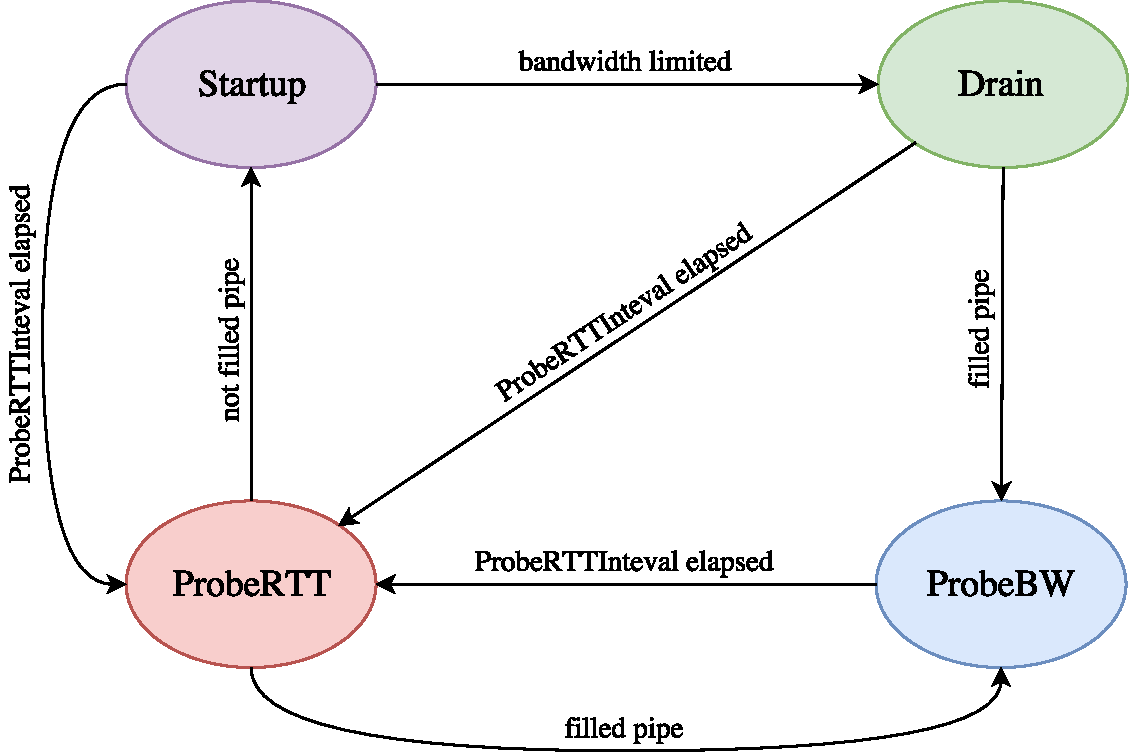
\includegraphics[scale=0.6]{chapters/bbr/img/state_diagram}

\end{figure}

Ricordiamo che gli obiettivi della state machine sono:

\begin{itemize}

\item Raggiungere il punto di massimo per il delivery rate, ed il punto di minimo per l'RTT;

\item Mantenere continuamente aggiornato il network path model, stimando sequenzialmente, nel corso del tempo, il bottleneck rate, ed il round trip propagation delay;

\item Garantire una equa suddivisione della capacità di rete, tra flussi BBR concorrenti;

\end{itemize}

Passiamo poi all'analisi degli stati, e delle transizioni.

\subsection{Startup}

Durante la fase di Startup, così com'era per il classico Slow Start, è d'interesse scovare subito il limite massimo del delivery rate. \bigskip

Ora considerando gli standard attuali, è ragionevole avere a che fare con 9 ordini di grandezza (1 Gbps), 10 ordini o 11 ordini di grandezza (10/100 Gbps). \bigskip

Pertanto è necessario che progressivamente ad ogni round, il sending rate perlomeno raddoppi. Ciò viene ottenuto configurando il pacing gain, ed il cwnd gain ad un valore pari al BBRHighGain (2/ln(2)). Ovvero la quantità di guadagno minima, che garantisce un raddoppio del tasso del mittente:

\begin{lstlisting}[caption=BBREnterStartup]
BBREnterStartup():
	BBR.state = Startup
	BBR.pacing_gain = BBRHighGain
	BBR.cwnd_gain = BBRHighGain

\end{lstlisting}

La fase di Startup termina nel momento in cui si riempie completamente la pipe. Ciò che tipicamente accade, e che non si riesce ad arrivare precisamente nel punto operativo, ma un pò aldilà, generando così delle code, di una quantità pari a (cwnd gain - 1) * BDP. \bigskip

Per individuare poi, in che momento si è saturato il delivery rate, viene usato il network path model.
Ciò che si fa è attendere, che per 3 round di fila, il bottleneck rate stimato non cresca più del 25\%. Quindi viene ricercato fondamentalmente un plateau per quest'ultimo. \bigskip

Motiviamo poi perchè siano necessari 3 round. Il primo round serve al destinatario, per effettuare l'auto-tuning della finestra di ricezione, sulla base dell'attuale capacità di rete. Il secondo round è usato dal mittente per riempire la finestra di ricezione. Il terzo, è quello in cui arriveranno i riscontri, per i pacchetti inviati, e cioè i sample che effettivamente sono indicativi del delivery rate.

\subsection{Drain}

Dopo una fase di Startup entriamo in Drain. Lo scopo di tale fase, è svuotare le code formate in precedenza. Ciò viene ottenuto in un round, invertendo il valore del pacing gain (così da lavorare con un sending rate < bottleneck rate):

\begin{lstlisting}[caption=BBREnterDrain]
BBREnterDrain():
	BBR.state = Drain
	BBR.pacing_gain = 1/BBRHighGain
	BBR.cwnd_gain = BBRHighGain

\end{lstlisting}

La fase di drain termina nel momento in cui la quantità di dati inflight arriva al valore attuale stimato del BDP. Quindi le code saranno tutte svuotate. \bigskip

A questo punto si passa in ProbeBW.

\subsection{ProbeBW} \label{ProbeBW}

Il BBR arriva nello stato ProbeBW, senza la presenza di code sul path di comunicazione. \bigskip

E' in questo stato, in cui il BBR spende la maggior parte del suo tempo. \bigskip

In ProbeBW, il BBR stima il bottleneck rate, operando in condizioni di massimo delivery rate, e ritardo di propagazione minimo. \bigskip

Ciò viene ottenuto attraverso una tecnica, chiamata gain cycling. Un gain cycle è tipicamente costituito da 8 fasi, in ognuna di queste fasi, il pacing gain viene impostato ad un valore utile a raggiungere le condizioni sopra espresse. \bigskip

I valori di pacing gain usati per ogni fase sono i seguenti: [5/4,3/4,1,1,1,1,1,1]. \bigskip

Partiamo dalla fase 0. In questa fase il pacing gain, porta il mittente, ad operare con un pacing rate > BtlBw. Questo serve ad ottenere campioni utili alla stima di quest'ultimo, in quanto è solo nella regione di bandwidth limited (figura \ref{Delivery_rate_round_trip_time}) ove il delivery rate $ \simeq $ bottleneck rate. \bigskip

La fase 0 dura almeno un RTprop, e termina nel momento in cui la quantità di dati inflight è pari a 5/4*BDP, o si verificano degli eventi di loss (non è possibile raggiungere la condizione inflight >= 5/4*BDP). \bigskip

Dopo la fase 0, l'obiettivo della fase 1, è drenare le code che sono state formate, impostando un valore di pacing rate di 3/4. Dunque in un tempo pari a RTprop, o prima (se le code si svuotano rapidamente), ci riportiamo nuovamente nel target point. \bigskip

Dopodichè dalla fase 2 in poi, il flusso opera nelle condizioni ideali, con un pacing gain pari a 1. \bigskip 

Proponiamo di seguito uno scenario reale di funzionamento del cycle gaining, in cui il bottleneck rate è di 10Mbps:

\begin{figure}[H]

\center
\caption{BBR probe bw gain cycling}
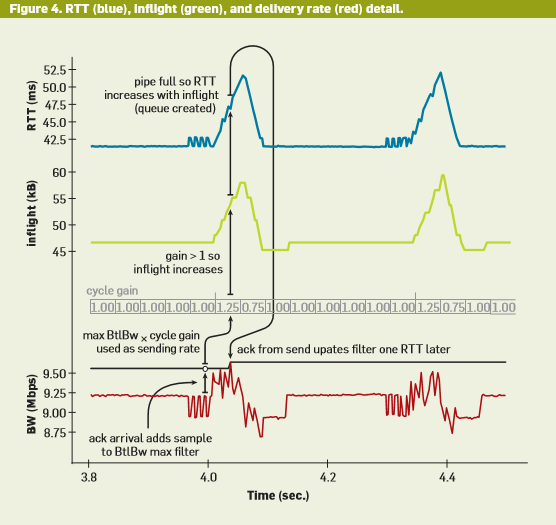
\includegraphics[scale=1.2]{chapters/bbr/img/probe_bw_gain_cycling}
\caption*{Figura tratta da \cite[p.~62]{Cardwell:2017:BCC:3042068.3009824}}

\end{figure}   
   
Aggiungiamo solo che in questo stato, la cwnd non ha un ruolo centrale, ed il suo target viene impostato a 2*BDP. Questo per non disturbare la modulazione del pacing rate, e per avere comunque un limite di sicurezza per l'inflight amout.

\subsection{ProbeRTT} \label{ProbeRTT}

Il BBR usa tale stato, per poter ottenere sample dell'RTT utili a stimare correttamente l'RTprop. \bigskip

Ogni ProbeRTTInterval (di una durata tipica di 10 s) il BBR transita in ProbeRTT, se la stima non è stata aggiornata. In tale stato ci si serve della cwnd per dare un colpo netto all quantità di dati inflight, impostandola al suo limite minimo (BBRMinCwndPipe). In questo modo, il flusso opera nella regione di application limited, ove non essendoci code, si otterrano sample dell'RTT $ \simeq $ RTprop. \bigskip

La cwnd è mantenuta a BBRMinCwndPipe, per un tempo pari al ProbeRTTDuration, che è circa 200 ms. Questa scelta permette di spendere solo il 2\% del tempo in ProbeRTT, dove il delivery rate è limitato fortemente, a discapito del 98\% speso, giustamente in ProbeBW. \bigskip

Allo scadere di un ProbeRTTDuration, viene ripristinata la cwnd, e si transita o in ProbeBW, o in Startup, a seconda dello stato attuale della rete.

\subsection{Evoluzione di un flusso BBR}

In conclusione possiamo dire che l'evoluzione di un flusso BBR, passa per un:

\begin{enumerate}

\item \textit{Warm up}: si passa in stati non stabili come Startup e Drain, per scovare velocemente il limite della banda di trasmissione;

\item \textit{Stati stabili}: quali ProbeBW e ProbeRTT, in cui il BBR aggiorna il proprio network path, ed imposta i propri parametri per raggiungere il target operating point;

\end{enumerate}

\begin{figure}[H]

\center
\caption{BBR state evolution}
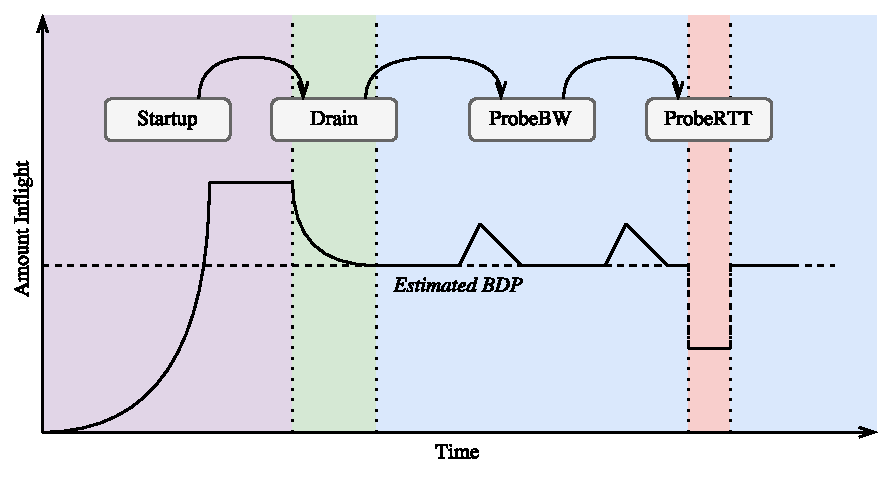
\includegraphics[scale=0.8]{chapters/bbr/img/bbr_evolution}

\end{figure}   


	\chapter{Casi reali d'impiego del BBR}
		\section{Cubic vs BBR}

Sia Cubic (App. A) che BBR, si servono di uno stato iniziale, quali lo Slow Start e lo Startup (rispettivamente), per scovare rapidamente il limite superiore del delivery rate. \bigskip

Tuttavia, hanno un intento differente, essendo due approcci al controllo di congestione diversi. \bigskip

Il Cubic cerca il limite superiore, per fissare la soglia di passaggio dallo Slow Start, al Congestion Avoidance. In cui semplicemente, continuerà ad aumentare il sending rate, ma in modo più lento. Questo finchè non raggiungerà il punto in cui scadrà un timeout, o il bottleneck buffer sarà saturo. Condizione in cui si verificheranno delle perdite. \bigskip

Il BBR invece, raggiunto il limite del delivery rate, con la consapevolezza di esser andato un pò oltre (il target point), e di aver generato delle code, passa in Drain per scaricarle.
Quindi arriva in ProbeBW, con le condizioni giuste e necessarie ad operare regolarmente al massimo tasso, ed ai minimi ritardi. \bigskip

Possiamo infatti sottolineare la loro evidente differenza nella gestione dell'RTT, con il seguente scenario:

\begin{figure}[H]

\center
\caption{First second of a 10Mbps, 40ms BBR flow}
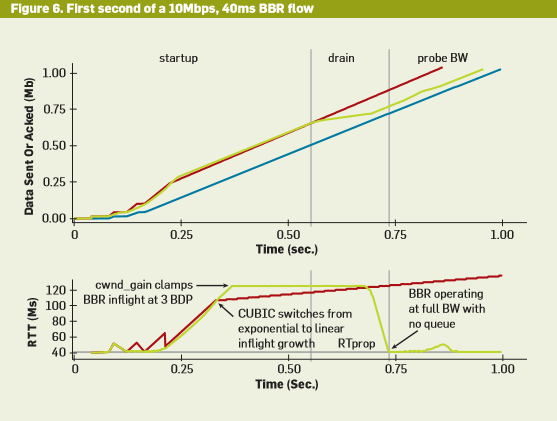
\includegraphics[scale=1.1]{chapters/4_application/img/start_cubic_bbr}
\caption*{Figura tratta da \cite[p.~63]{Cardwell:2017:BCC:3042068.3009824}}

\end{figure}

L'ambito operativo di Cubic, è sicuramente quello peggiore. In quanto avremo dei livelli alternati di RTT, tra il 70\% ed il 100\% (con 0\% intendiamo la condizione in cui RTT $ \simeq $ RTprop), ed un delivery rate si al massimo, ma dimezzato ogni volta in corrispondenza di una perdita (o abbattuto ad un timeout):

\begin{figure}[H]

\center
\caption{First eight seconds of a 10Mbps, 40ms cubic and BBR flow}
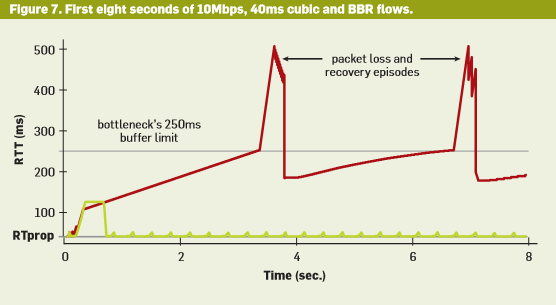
\includegraphics[scale=1.1]{chapters/4_application/img/rtt_cubic_bbr}
\caption*{Figura tratta da \cite[p.~64]{Cardwell:2017:BCC:3042068.3009824}}

\end{figure}

Bisogna però prendere atto di una cosa, ovvero che Cubic a differenza del BBR non dispone di un network path model. Quindi non è possibile contenere l'RTT se non lo si traccia nel tempo, e se non è quest'ultimo a determinare il valore dei parametri di controllo della soluzione.

\section{Fairness tra flussi BBR}

Tra flussi BBR concorrenti, il livello di fairness raggiunto, testimoniato anche da appositi esperimenti, è molto soddisfacente. \bigskip

Ecco infatti un caso d'esempio di 5 flussi concorrenti, che condividono un bottleneck link da 100 Mbps, ed un RTT da 10 ms:

\begin{figure}[H]

\center
\caption{Throughput of five BBR flows sharing a bottleneck}
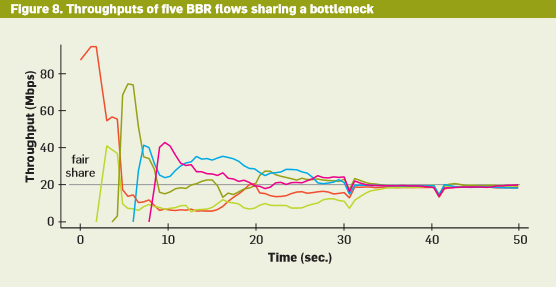
\includegraphics[scale=1.1]{chapters/4_application/img/fairness_bbr}
\caption*{Figura tratta da \cite[p.~64]{Cardwell:2017:BCC:3042068.3009824}}

\end{figure}

Nella figura viene presentato uno scenario abbastanza generale, in cui i flussi BBR non nascono tutti nello stesso istante. \bigskip

Ciò che ci aspettiamo accada è semplice. Nello stato di ProbeBW i flussi al di sopra del fair share, scopriranno un calo del bottleneck rate. Quindi si accorgeranno della perdita di banda, riconfigurando poi il loro pacing rate. \bigskip

Andando poi avanti, quando (di nuovo) un flusso al di sopra del fair share - che dunque sta generando un maggior traffico - entrerà in ProbeRTT, svuoterà considerevolmente il bottleneck buffer. Ciò porterà ad un aggiornamento dell'RTprop degli altri flussi concorrenti. \bigskip

Alla lunga, il tutto porta a sincronizzare l'entrata nello stato di ProbeRTT, di tutti i flussi. Così tutti portranno stimare il reale valore dell'RTprop, così come del bottleneck rate.

\section{Fairness tra flussi loss-based e BBR}

In questo caso, è abbastanza (purtroppo) prevedibile, che allo stato attuale delle cose, sia difficile raggiungere una suddivisione equa della banda. \bigskip

Fondamentalmente, un flusso loss-based presenta un andamento del throughput, pressochè a dente di sega:

\begin{figure}[H]

\center
\caption{TCP loss-based evoluzione del throughput}
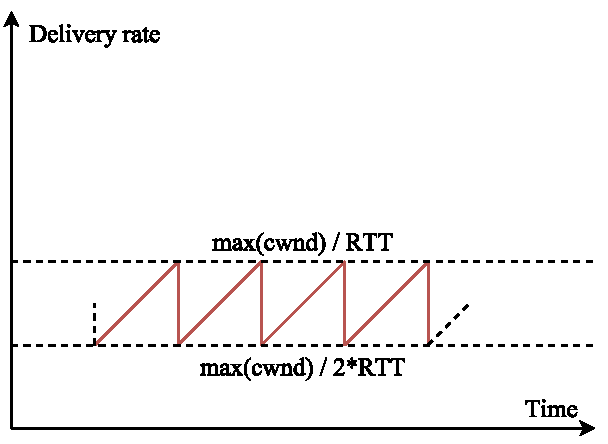
\includegraphics[scale=0.8]{chapters/4_application/img/tcp_reno}

\end{figure}

Allora ci aspetteremo che un flusso BBR, abbia maggiore banda, nelle fasi di low-throughput del flusso loss, mentre questi diminuisca quando quest'ultimo arriva al suo massimo (le sue reali possibilità). Tuttavia, un flusso loss, ad esempio come Reno, raggiunge il massimo in corrispondenza di un evento di perdita, per cui non manterrà a lungo tale livello. \bigskip

Per la consultazione di appositi esperimenti si veda \cite{ietf:ietf-98-bbr-slides}. 

\section{Rete Google B4}

B4 è una rete proprietaria ad estensione geografica, dalle alte performance, di Google. \bigskip

Nel 2015, quando BBR non era più solo una teoria, ma una idea concreta, si diede inizio ad una transizione verso quest'ultimo. Così nel 2016, Cubic è stato completamente sostituito dal BBR, che non essendo un approccio loss-based, ha portato un notevole incremento delle prestazioni. \bigskip

Il primo artefatto d'analisi, mette a rapporto il throughput raggiunto con BBR rispetto quello raggiunto con Cubic:

\begin{figure}[H]

\center
\caption{BBR vs CUBIC relative throughput improvement}
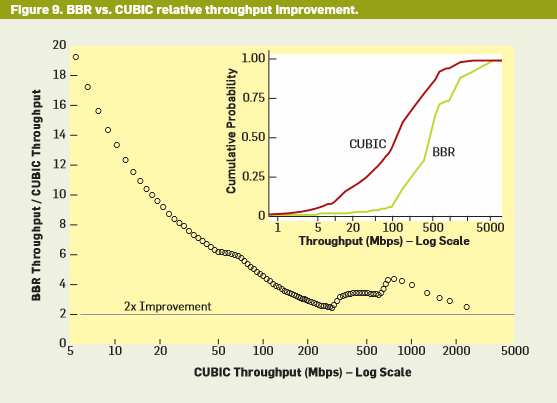
\includegraphics[scale=1]{chapters/4_application/img/bbr_vs_cubic_1}
\caption*{Figura tratta da \cite[p.~64]{Cardwell:2017:BCC:3042068.3009824}}

\end{figure}

Tali dati, raccolti da varie sonde, disposte in vari punti della rete B4, mettono in evidenza un incremento prestazionale che va dal 2x al 25x. In realtà, l'incremento del BBR è mascherato dal limite imposto ai buffer di ricezione TCP (8 MB). \bigskip

Alzando tale limite è stato ottenuto, su un path tra Europa e USA, un throughput di 2 Gbps, contro i 15 Mbps di Cubic. Parliamo di un incremento: 133x. \bigskip

Nel grafico vengono anche messe a confronto le distribuzioni di probabilità cumulative. Da esso possiamo notare (qualitativamente) che:

\begin{table}[H]

\centering
\caption{Throughput CDF}	

\begin{tabular}{ccc}

\toprule
 & BBR & Cubic \\
\midrule
P(thput < 1) & $ \simeq $ 0 & $ \simeq $ 0 \\
\midrule
P(thput < 20) & $ \simeq $ 0 & 0.19  \\
\midrule
P(thput < 100) & 0.06 & 0.5 \\
\midrule
P(thput < 500) & 0.62 & 0.87  \\
\midrule
P(thput < 5000) & 1 & 1  \\
\bottomrule

\end{tabular}
\end{table}

Il secondo artefatto mette a confronto il throughput utile sostenibile, in funzione del loss-rate:

\begin{figure}[H]

\center
\caption{BBR vs CUBIC goodput under loss}
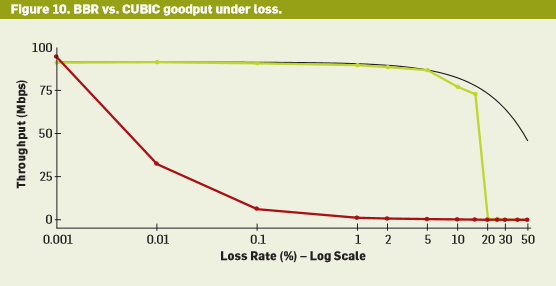
\includegraphics[scale=1]{chapters/4_application/img/bbr_vs_cubic_loss_rate}
\caption*{Figura tratta da \cite[p.~65]{Cardwell:2017:BCC:3042068.3009824}}

\end{figure}

Ricordando che un loss-rate ragionevole è circa dell'1\%, e notando che il BBR perde performance tra 5\% ed 20\%, questo è un ottimo miglioramento.

%\section{Youtube}
	
	\chapter{Note}	
		Tutto lo pseudo-codice presente nella relazione, è tratto dagli internet draft:

\begin{itemize}

\item \cite{ietf:draft-cardwell-iccrg-bbr-congestion-control-00}
\item \cite{ietf:draft-cheng-iccrg-delivery-rate-estimation-00}

\end{itemize}

	
	\printbibliography

	%\bibliographystyle{plain}
	%\bibliography{bibliografia} 

\end{document}